\section{详细设计}

\subsection{主要界面预览}
\begin{figure}[H]
    \centering
    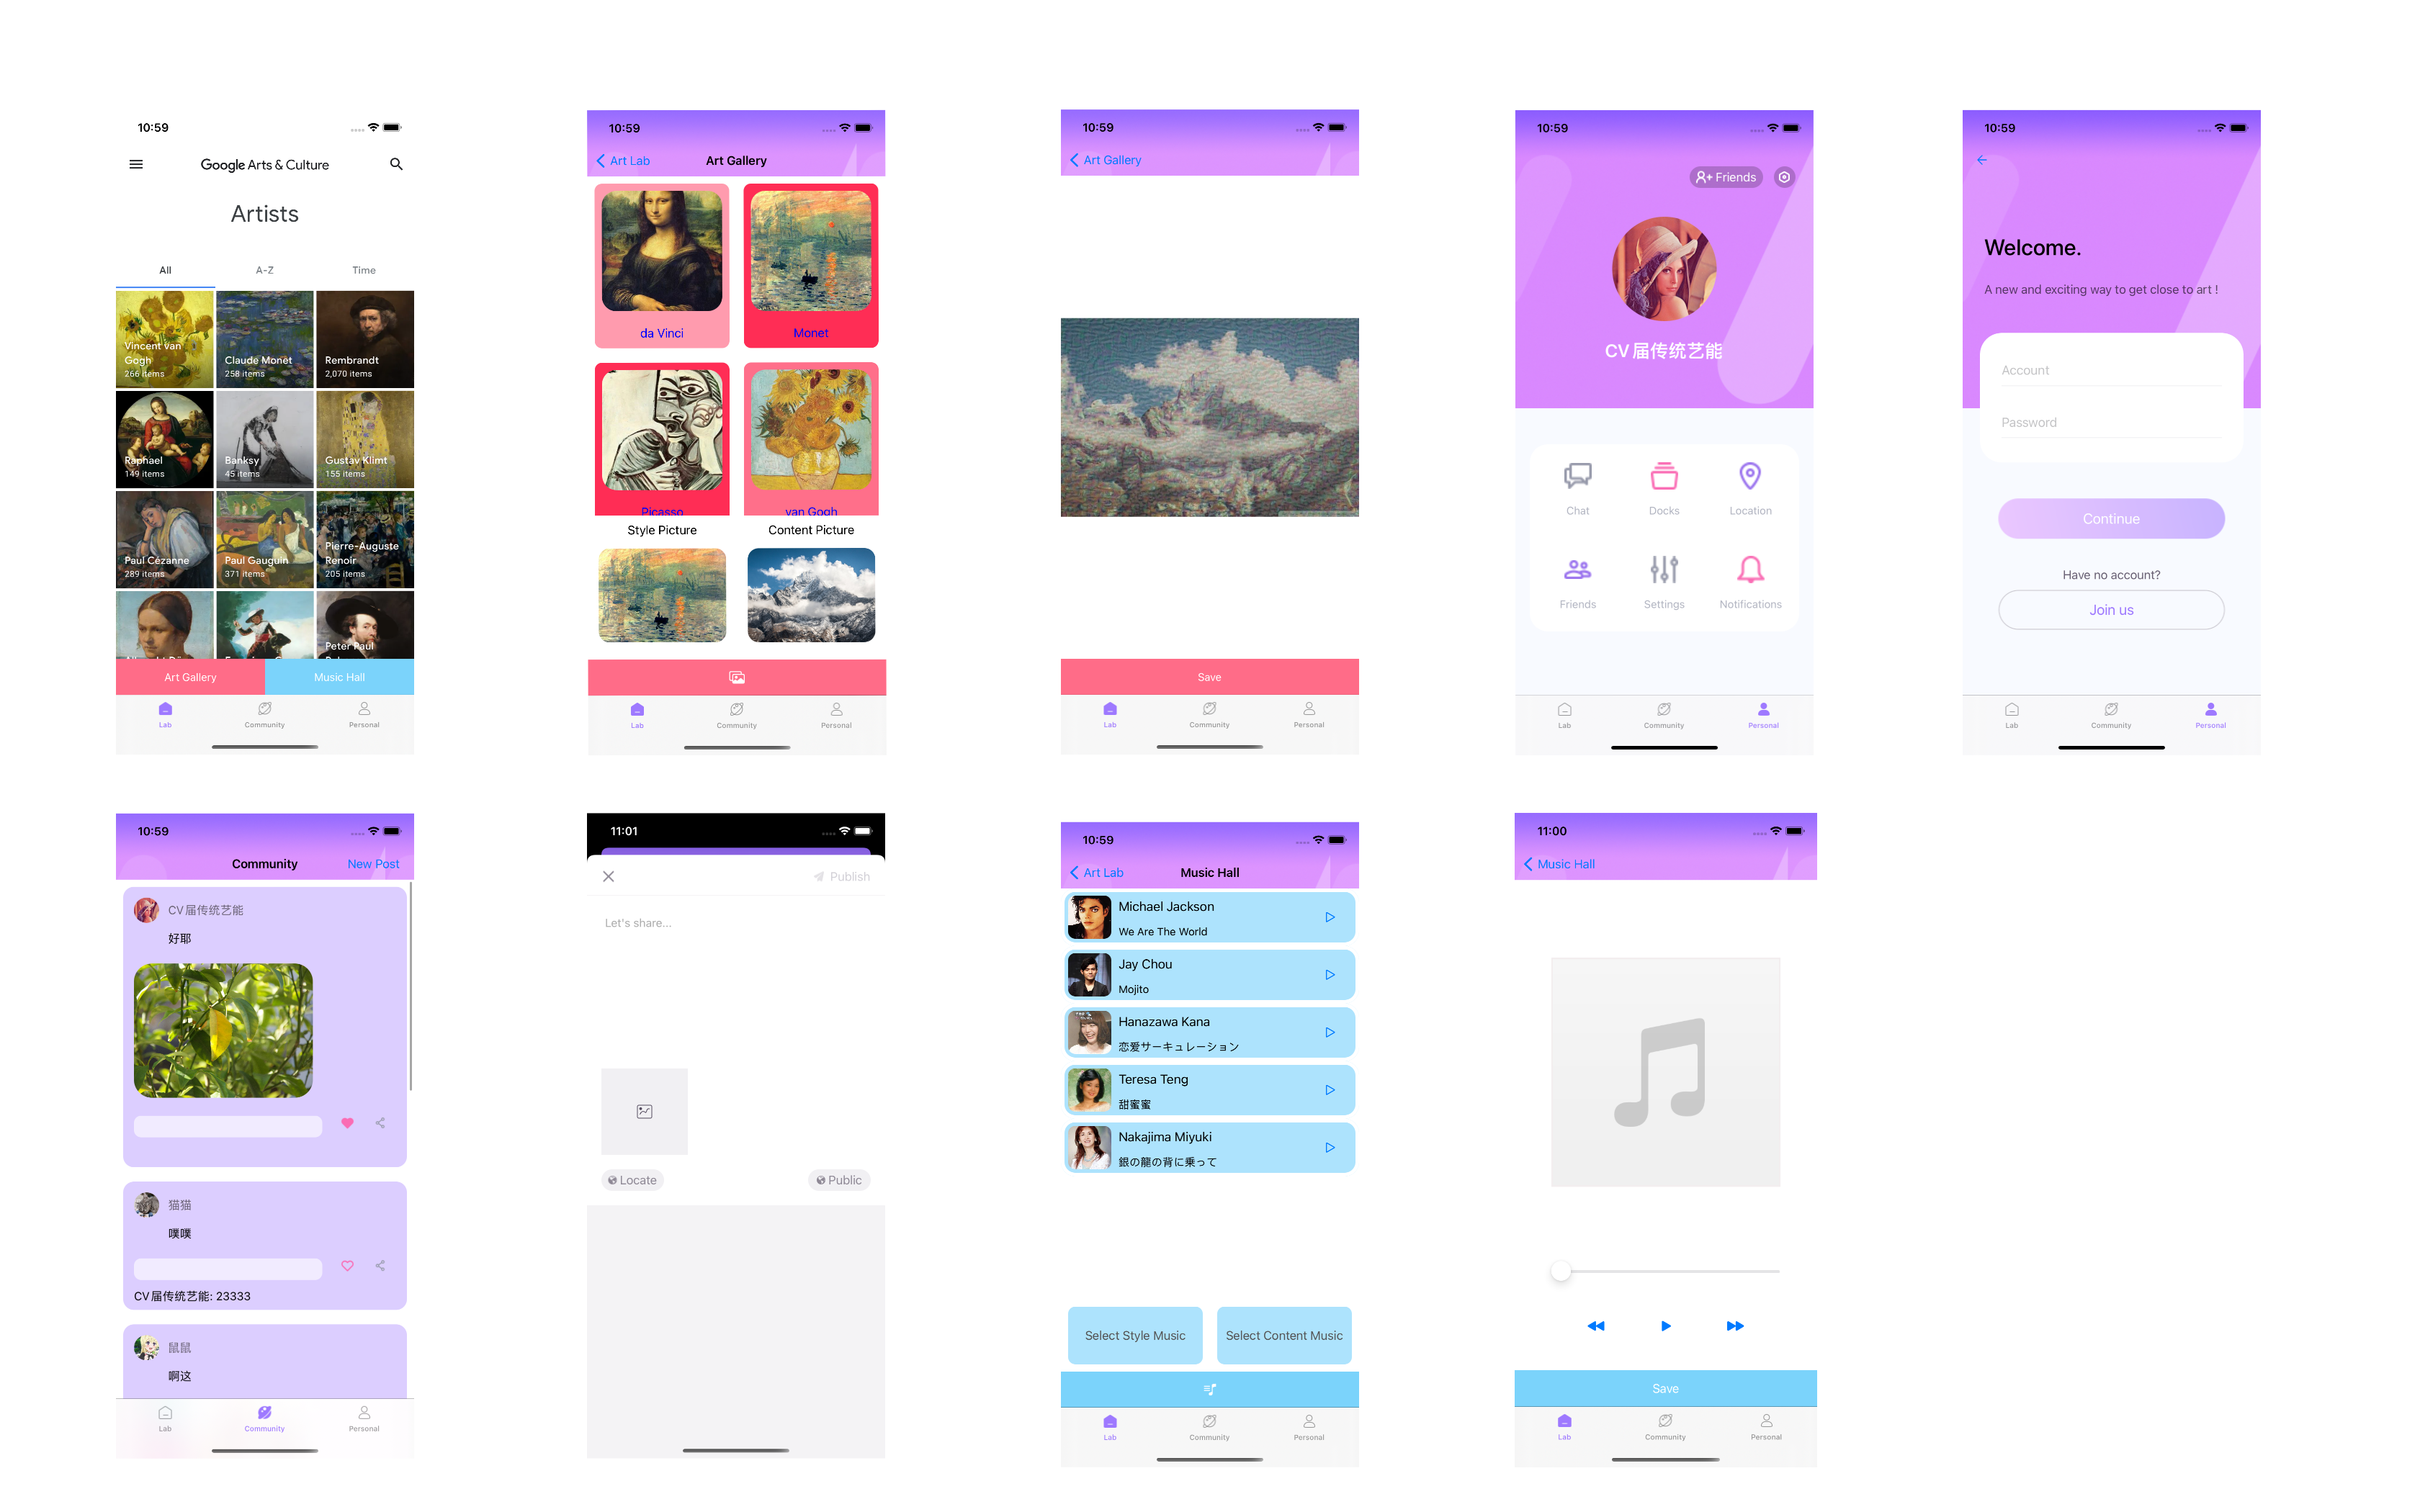
\includegraphics[width=
    \textwidth]{figures/预览}
    \caption{登陆界面示意图}
    \label{fig:my_label}
\end{figure}

\subsection{移动端详细设计}


移动端的主要任务是构建 App 界面,实现事件交互,后端通信等。本 App 使用 UIKit 框架,基于 Swift 和 Objective-C 语言开发。使用的主要第三方库如下:

\begin{itemize}
	\item \textbf{AFNetworking} \ iOS 著名网络框架
	\item \textbf{SocketRocket} \ Facebook 开源的 WebSocket 协议通信框架
	\item \textbf{SAMKeychain} \ 隐私信息存储管理框架
	\item \textbf{SVProgressHUD} \ 信息、进度提示框架
\end{itemize}

\subsubsection{实验室}

\begin{wrapfigure}{l}{4.5cm}
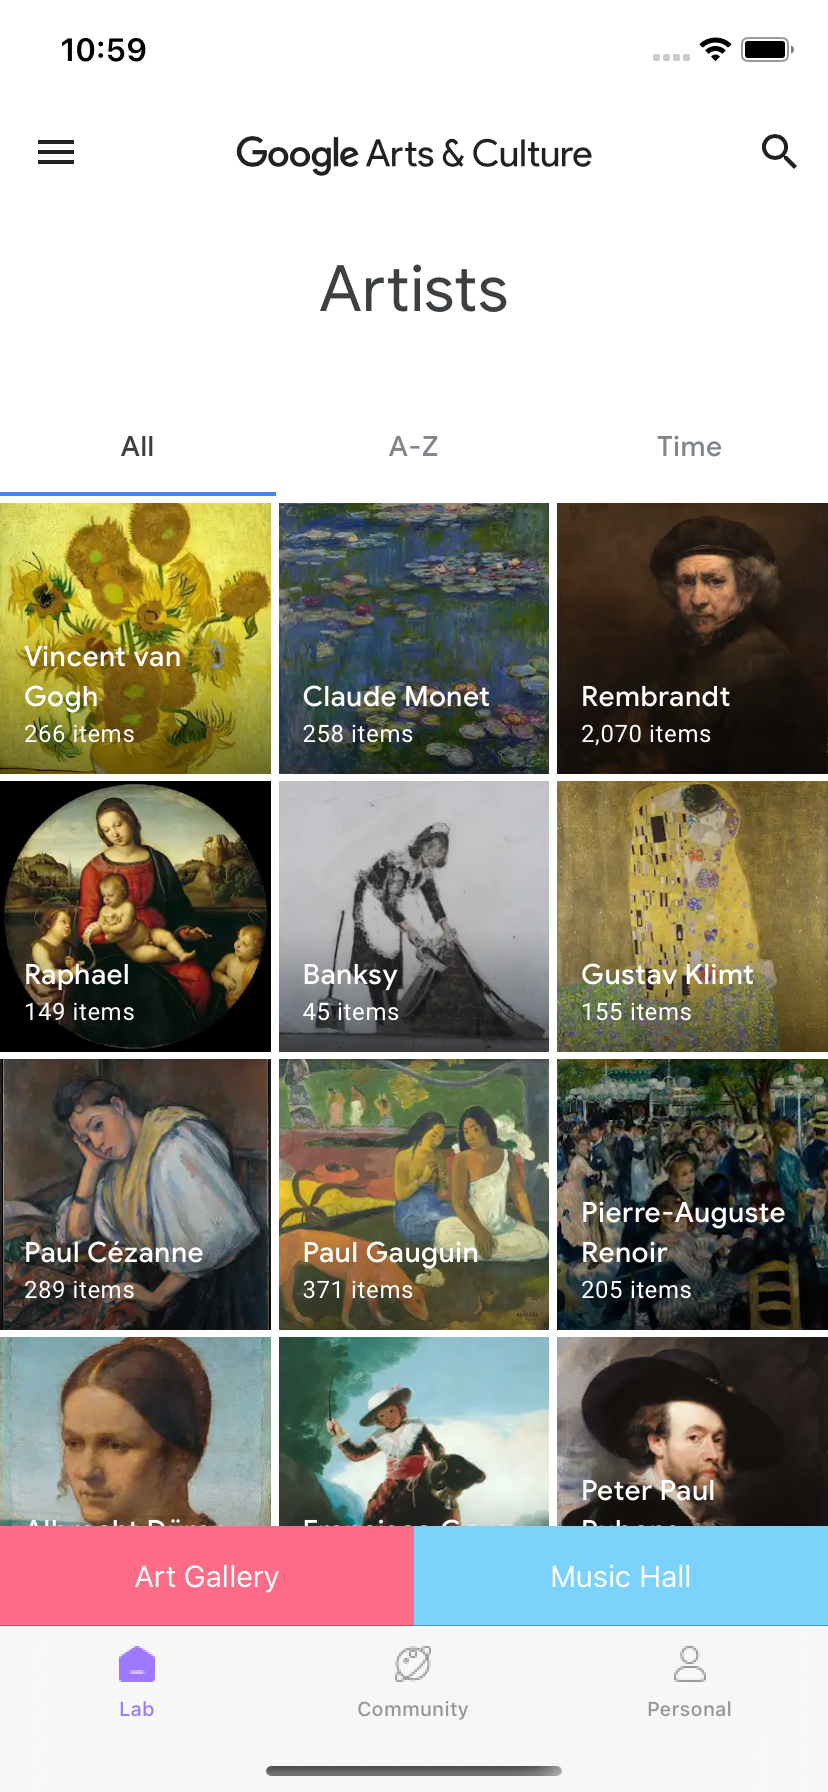
\includegraphics[width=4cm]{figures/主页.png}
\caption{主页示意图}
\label{fig:my_label}
\end{wrapfigure}

这一界面提供了一些艺术家及其作品的展示,以及图像和音乐风格转换的入口。

\subsubsection{图像风格转换}

\begin{wrapfigure}{l}{4.5cm}
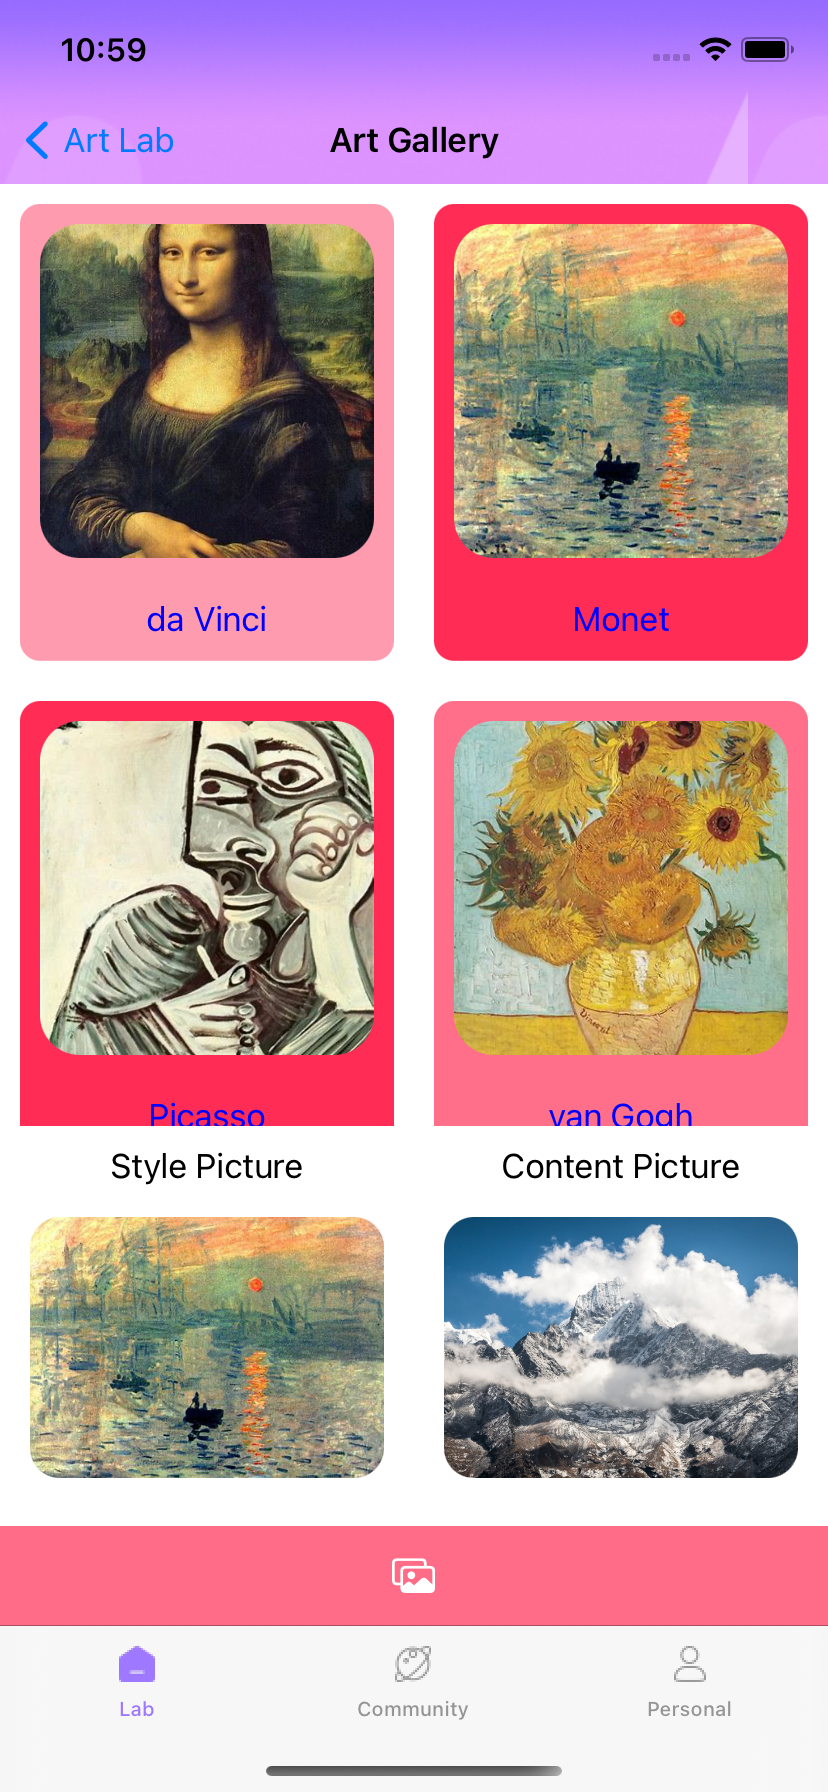
\includegraphics[width=4cm]{figures/图片风格转换.png}
\caption{图片风格转换示意图}
\label{fig:my_label}
\end{wrapfigure}


这一界面可以选择想要转换的风格图片和内容图片,并在上半部提供了一些预设的风格图片。下方的两个按钮可以选择的样式和内容图片,选择的图片会在按钮上显示出来。点击底部的按钮后即可跳转到转换结果界面。

\begin{wrapfigure}{l}{4.5cm}
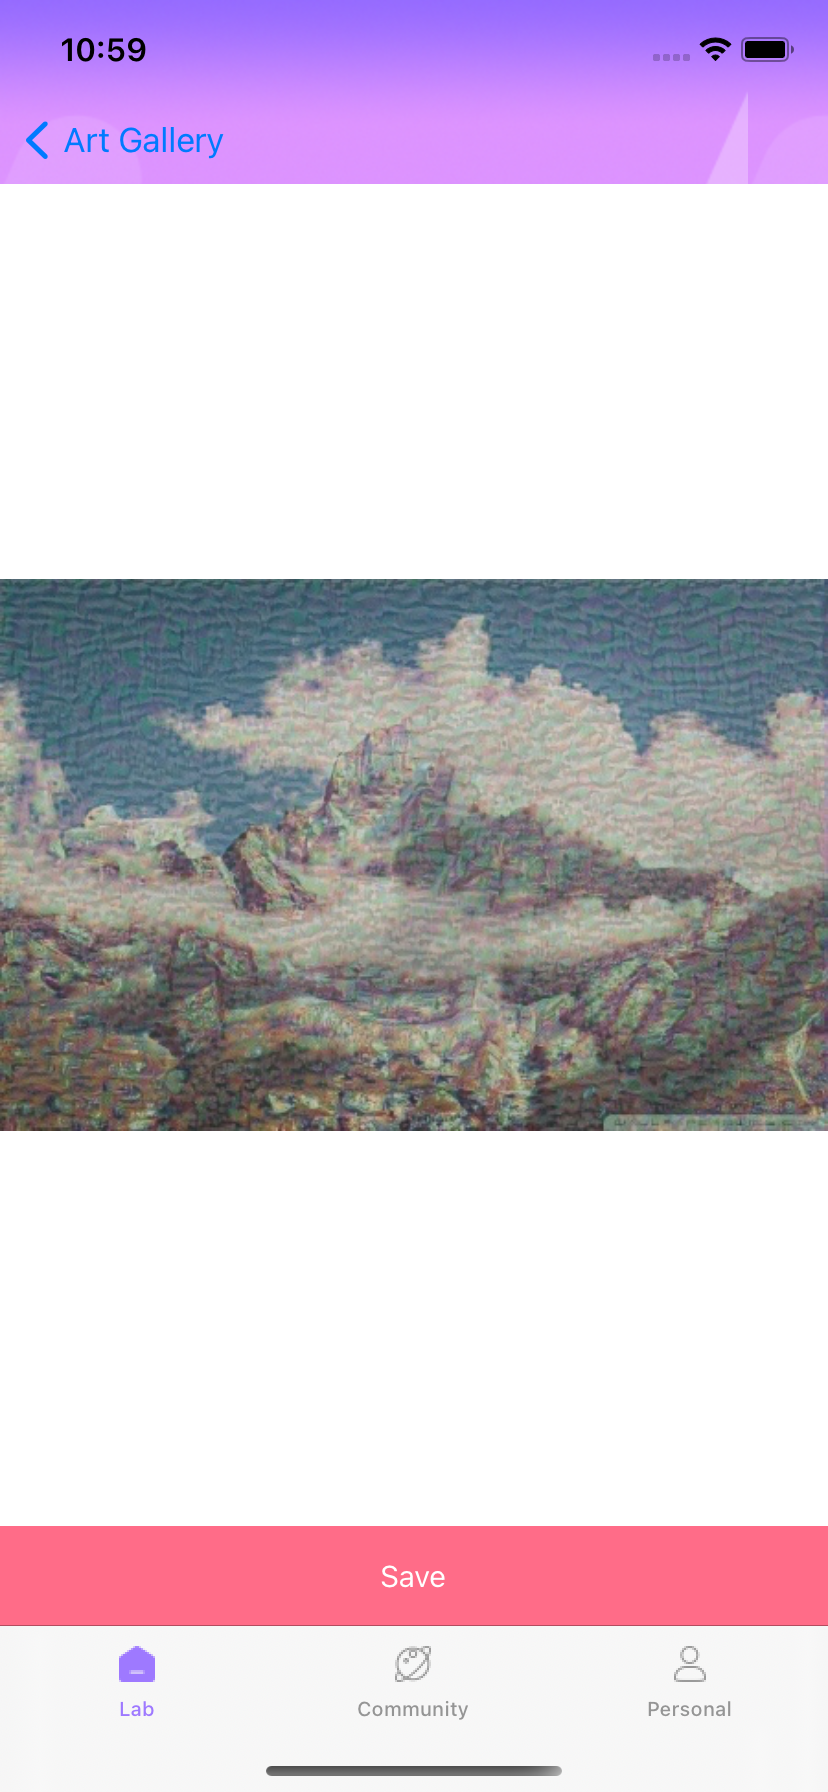
\includegraphics[width=4cm]{figures/图片转换效果.png}
\caption{转换结果示意图}
\label{fig:my_label}
\end{wrapfigure}

这一界面展示了转换好风格的图片,下方有一个按钮可以保存图片到相册。在此页面加载时,App 向服务器发送请求,建立 WebSocket 连接,实现 App 与服务器间的双向通信。App 向服务器发送风格图片和内容图片,服务器转换完成后,向 App 发送转换好的图片,App 收到后在 UI 界面上显示此图片,并断开与服务器的连接。

\subsubsection{音乐风格转换}

%\begin{figure}[H]
%    \centering
%    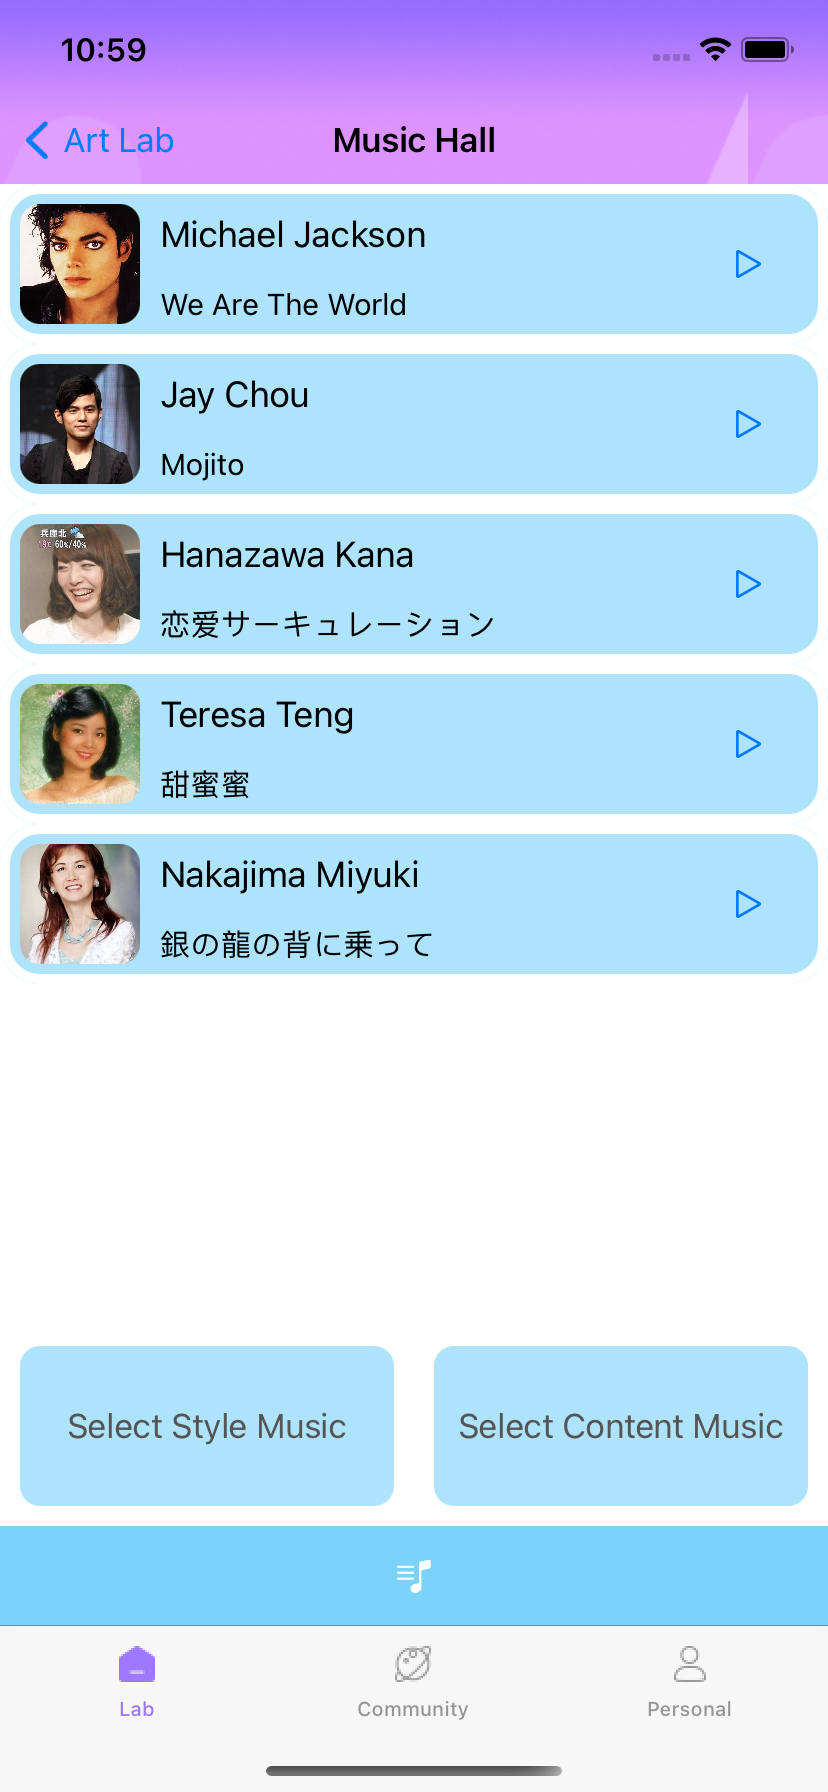
\includegraphics[width=0.5
%    \textwidth]{figures/音乐风格转换.png}
%    \caption{音乐风格转换示意图}
%    \label{fig:my_label}
%\end{figure}

\begin{wrapfigure}{l}{4.5cm}
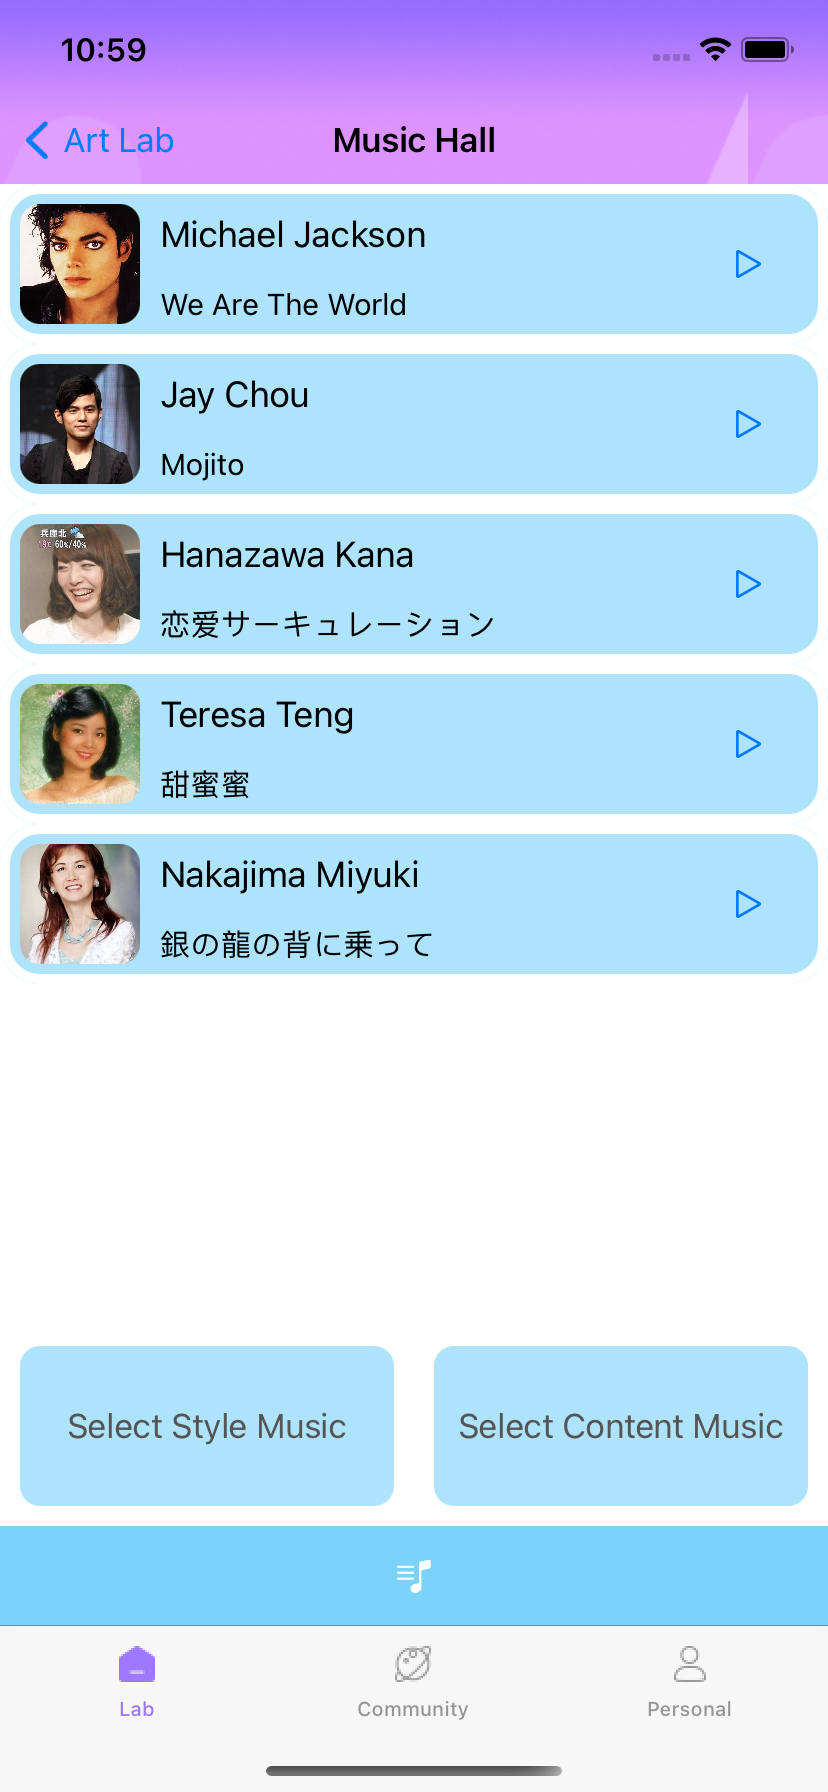
\includegraphics[width=4cm]{figures/音乐风格转换.png}
\caption{音乐风格转换示意图}
\label{fig:my_label}
\end{wrapfigure}

这一界面可以选择想要转换的风格音乐和内容音乐,并在上半部提供了一些预设的风格音乐。下方的两个按钮可以选择的样式和内容音乐,选择的音乐文件名会在按钮上显示出来。点击底部的按钮后即可跳转到转换结果界面。


%\begin{figure}[H]
%    \centering
%    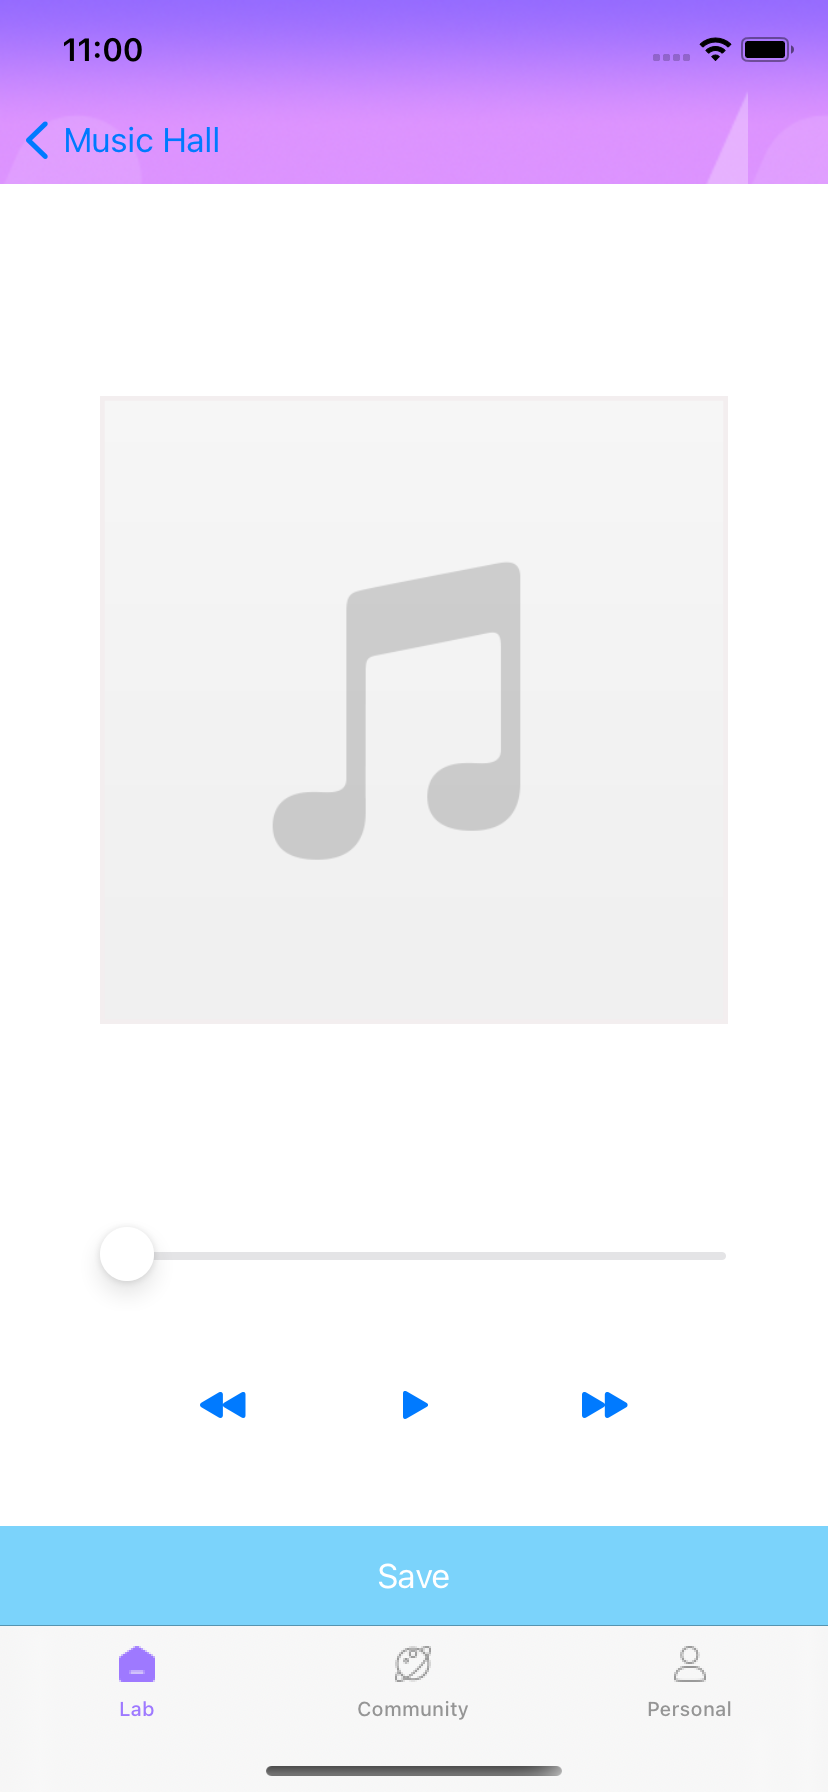
\includegraphics[width=0.5
%    \textwidth]{figures/音乐试听.png}
%    \caption{播放音乐示意图}
%    \label{fig:my_label}
%\end{figure}

\begin{wrapfigure}{l}{4.5cm}
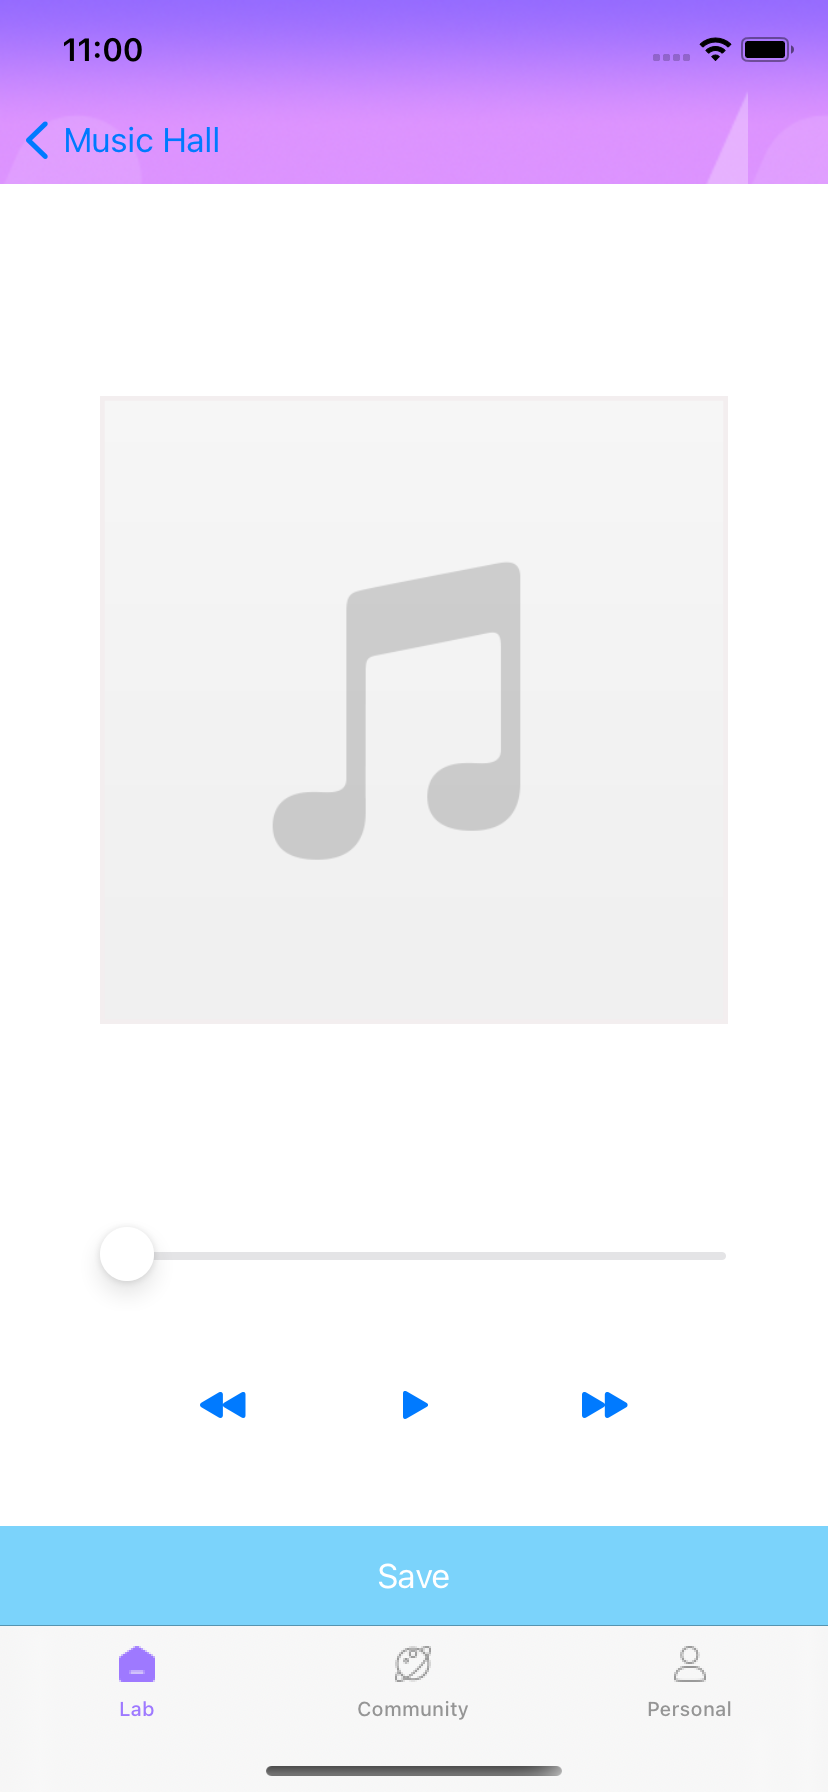
\includegraphics[width=4cm]{figures/音乐试听.png}
\caption{播放音乐示意图}
\label{fig:my_label}
\end{wrapfigure}

这一界面实现了一个简单的播放器,包括播放/暂停按钮,前进/后退按钮,可以拖动的进度条,以提供转换好的音频文件的试听。下方的按钮可以保存音频文件到 iOS 系统的文件应用中。

\subsubsection{社区}

%\begin{figure}[H]
%    \centering
%    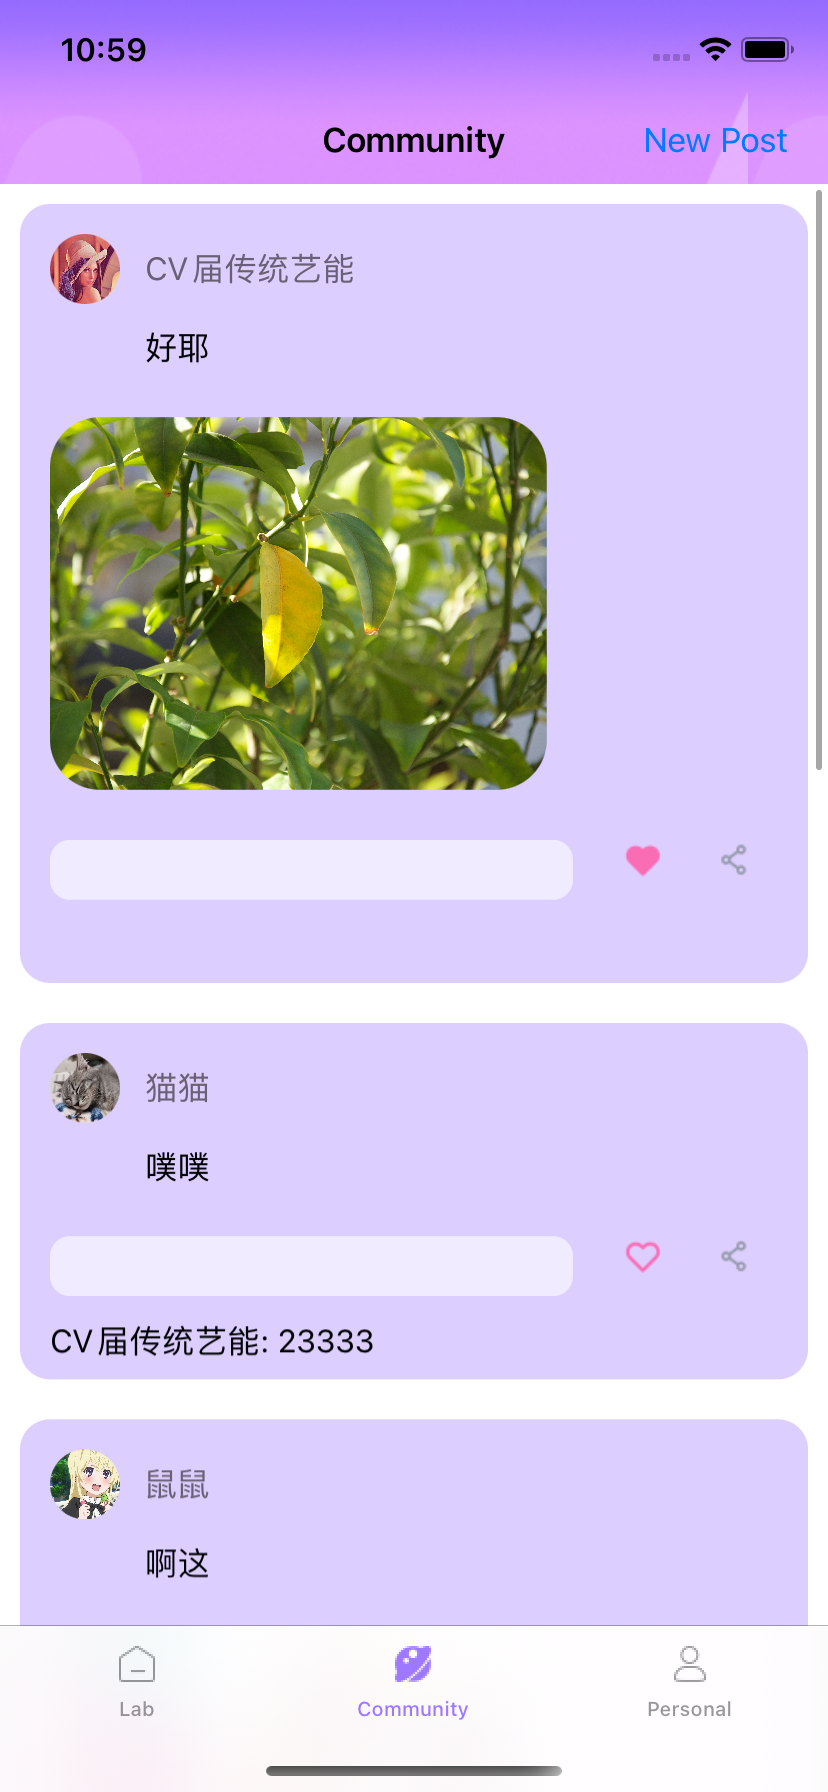
\includegraphics[width=0.5
%    \textwidth]{figures/社区.png}
%    \caption{社区示意图}
%    \label{fig:my_label}
%\end{figure}

\begin{wrapfigure}{l}{4.5cm}
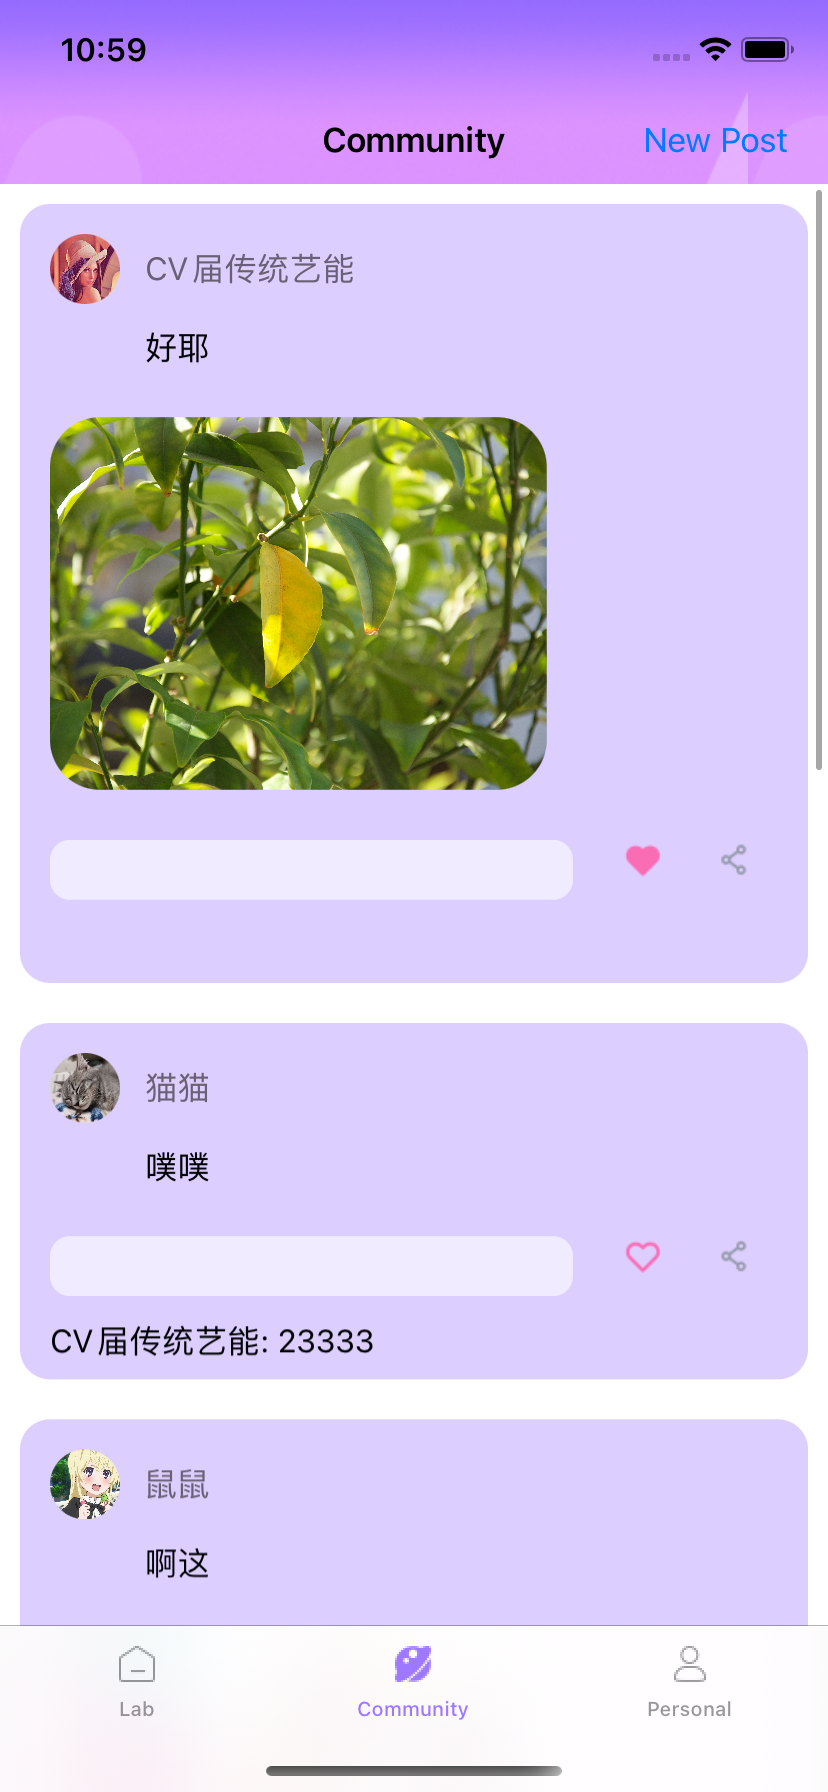
\includegraphics[width=4cm]{figures/社区.png}
\caption{社区示意图}
\label{fig:my_label}
\end{wrapfigure}


这一界面可以浏览时间线上的帖子,右上角有发贴按钮,可以点击进入发贴界面。

%\begin{figure}[H]
%    \centering
%    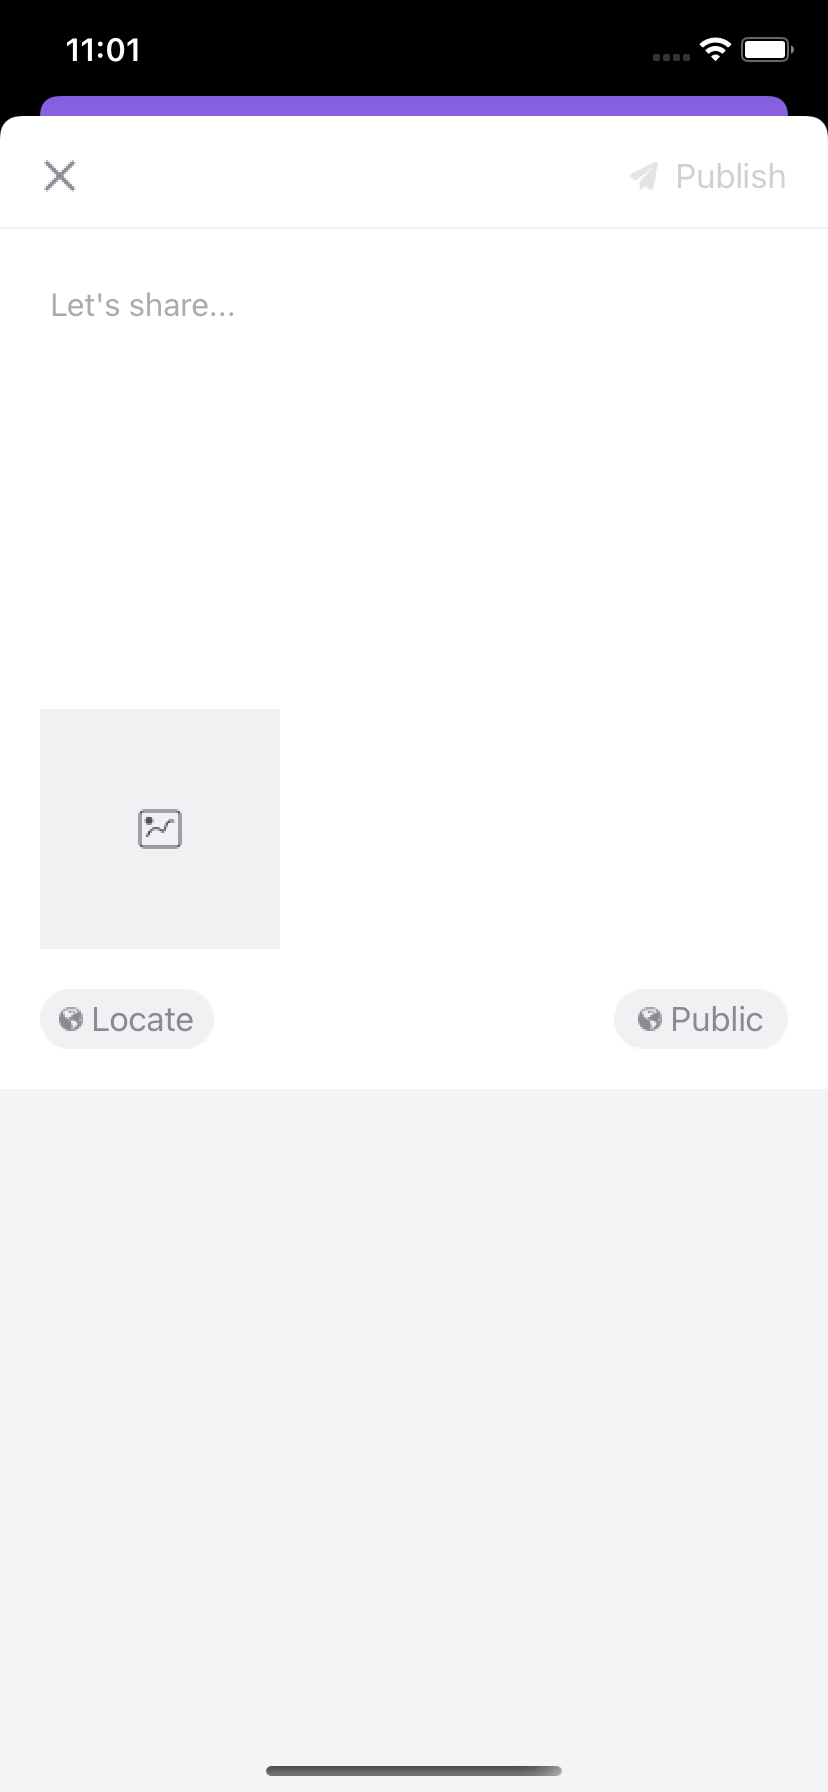
\includegraphics[width=0.5
%    \textwidth]{figures/发贴.png}
%    \caption{发帖示意图}
%    \label{fig:my_label}
%\end{figure}

\begin{wrapfigure}{l}{4.5cm}
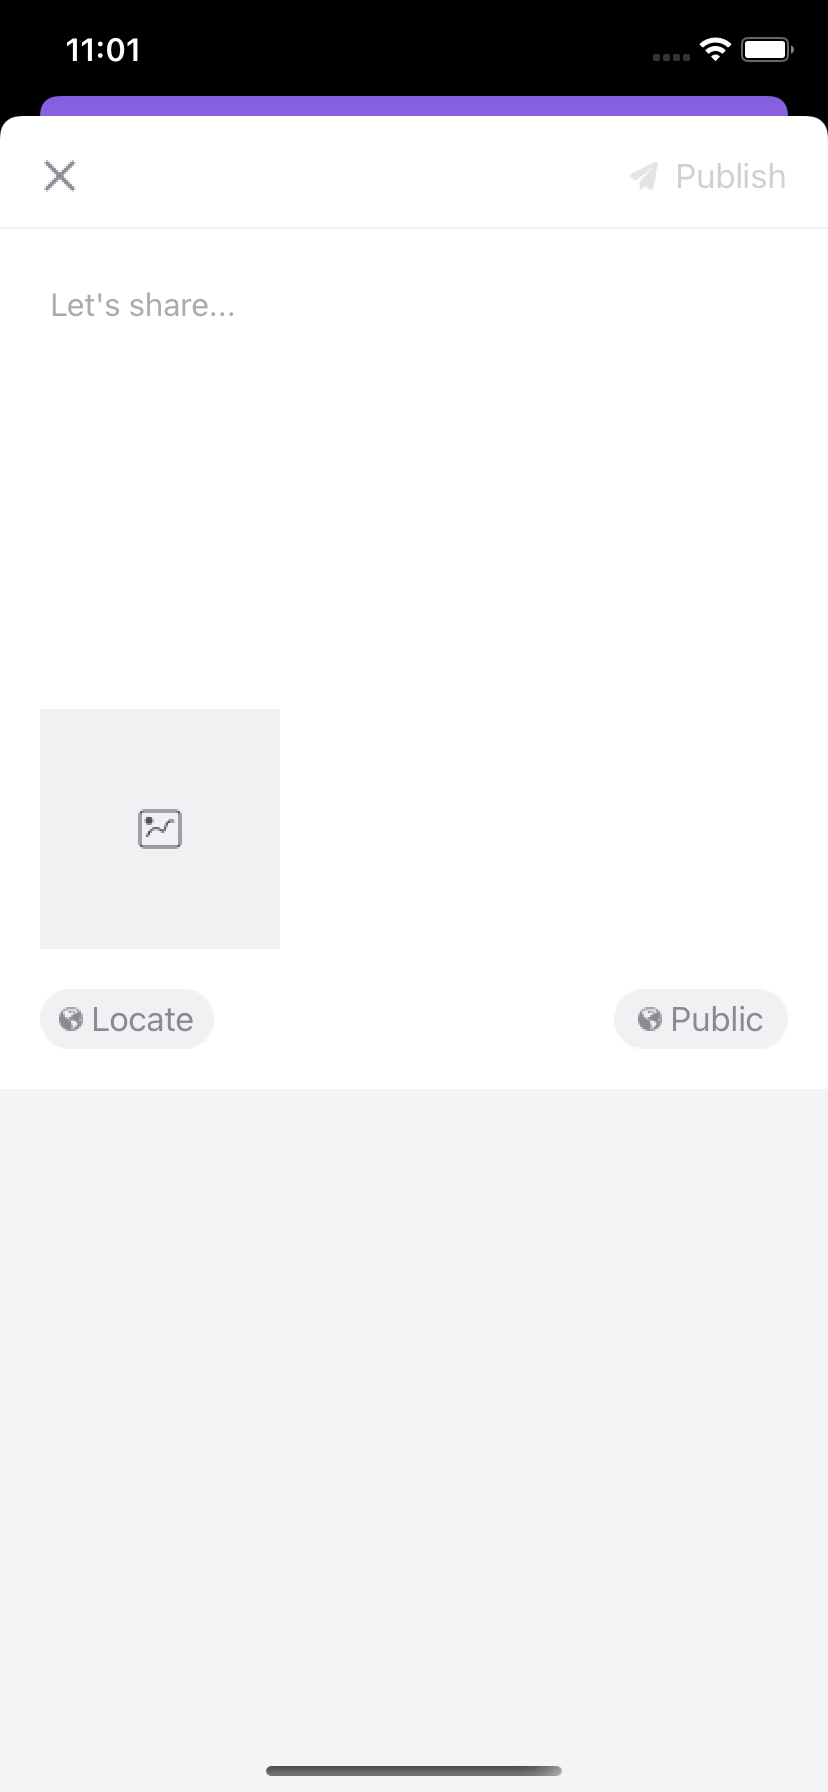
\includegraphics[width=4cm]{figures/发贴.png}
\caption{发帖示意图}
\label{fig:my_label}
\end{wrapfigure}

这一界面可以进行发帖操作,发帖内容支持文字、图片和音频。

\subsubsection{个人信息}

%\begin{figure}[H]
%    \centering
%    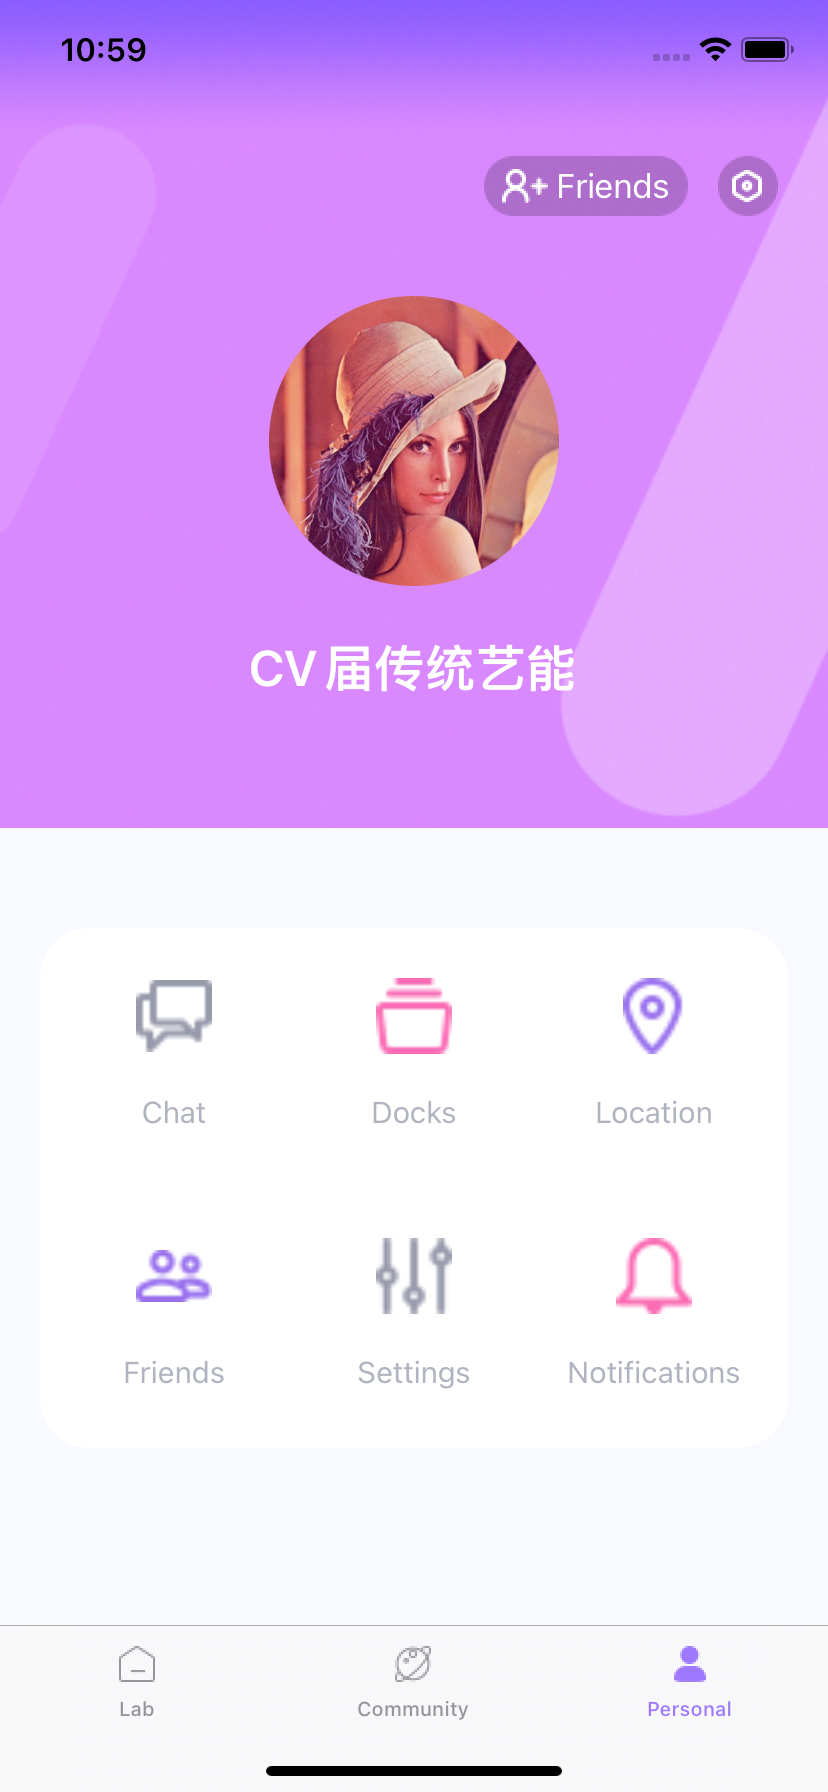
\includegraphics[width=0.5
%    \textwidth]{figures/用户.png}
%    \caption{用户示意图}
%    \label{fig:my_label}
%\end{figure}

\begin{wrapfigure}{l}{4.5cm}
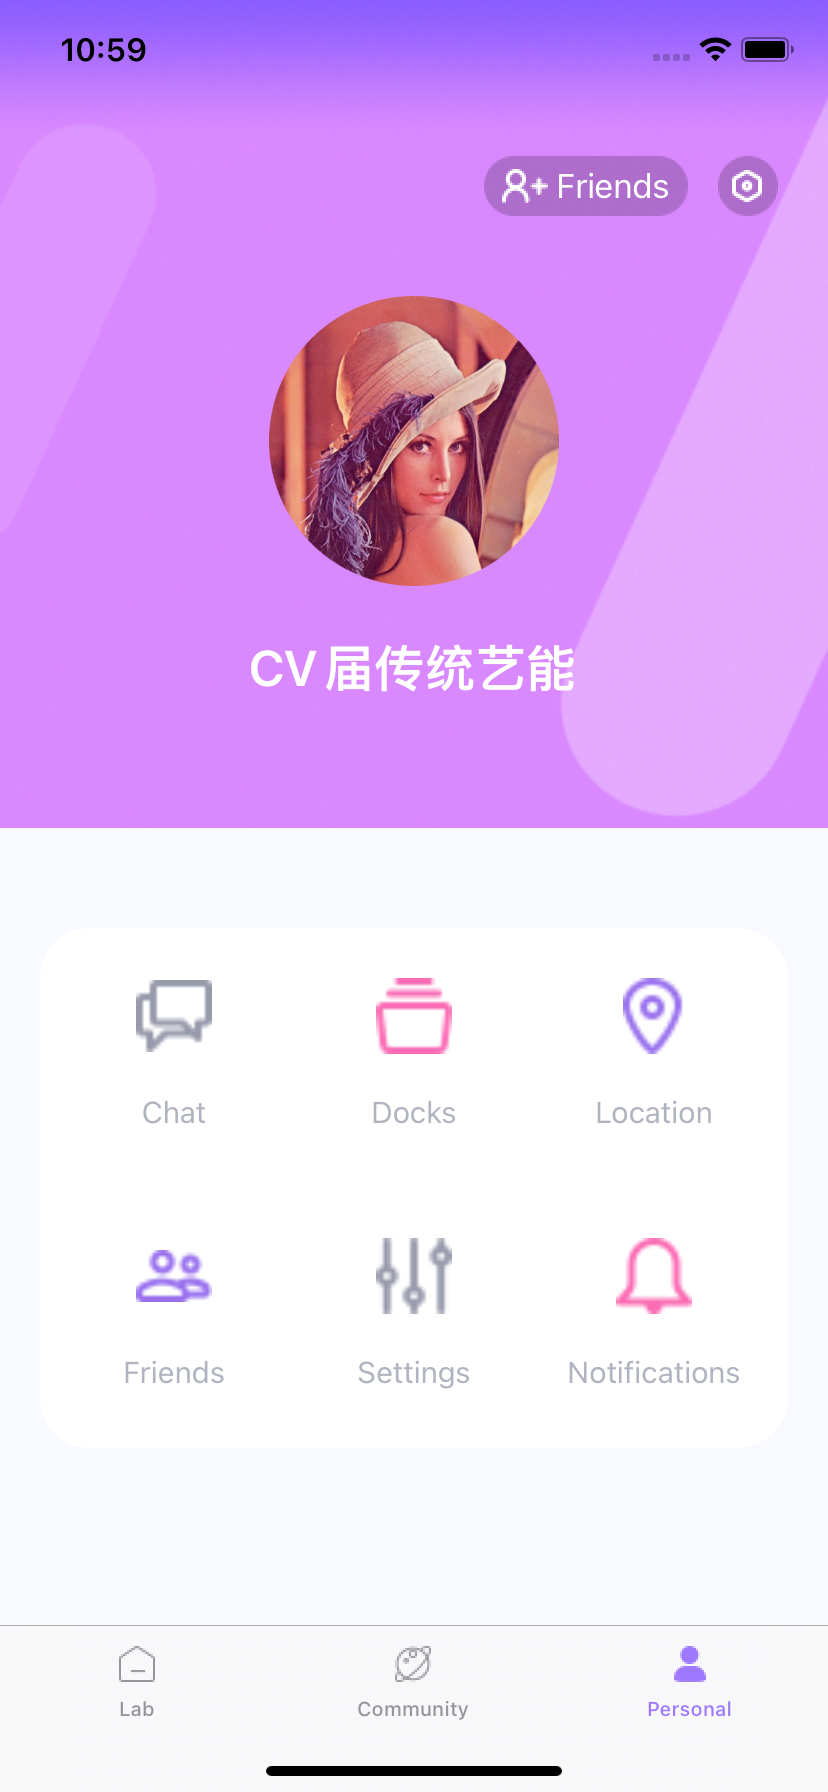
\includegraphics[width=4cm]{figures/用户.png}
\caption{用户示意图}
\label{fig:my_label}
\end{wrapfigure}


这一界面可以显示用户的个人信息,如头像,昵称,自己的作品,收藏和设置。


%\begin{figure}[H]
%    \centering
%    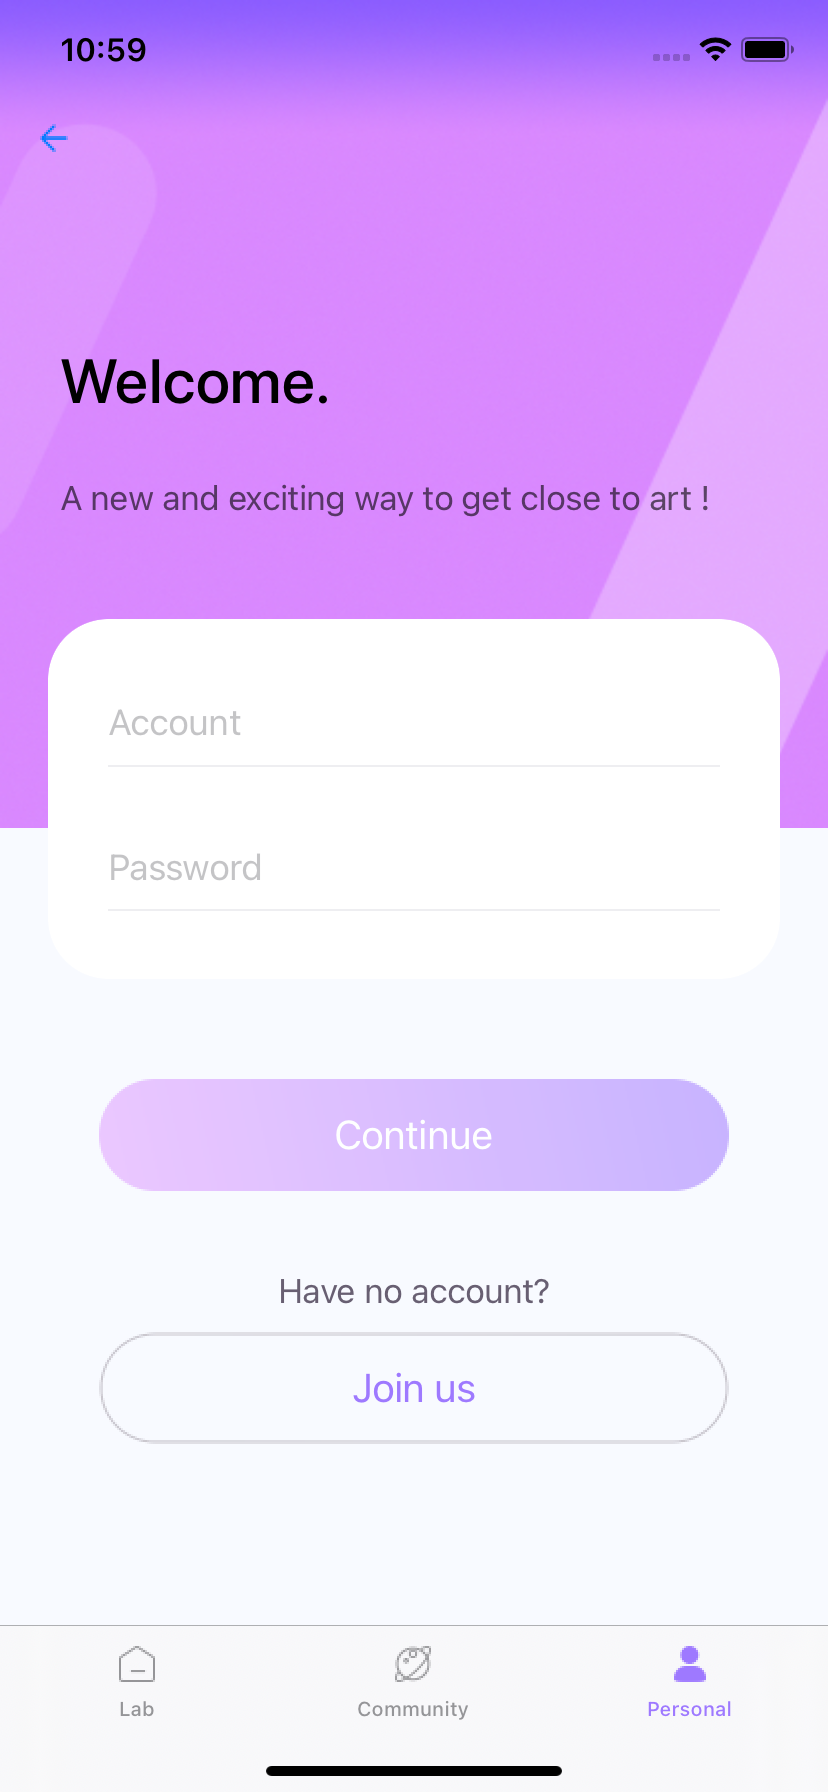
\includegraphics[width=0.5
%    \textwidth]{figures/登录.png}
%    \caption{登陆示意图}
%    \label{fig:my_label}
%\end{figure}

\begin{wrapfigure}{l}{4.5cm}
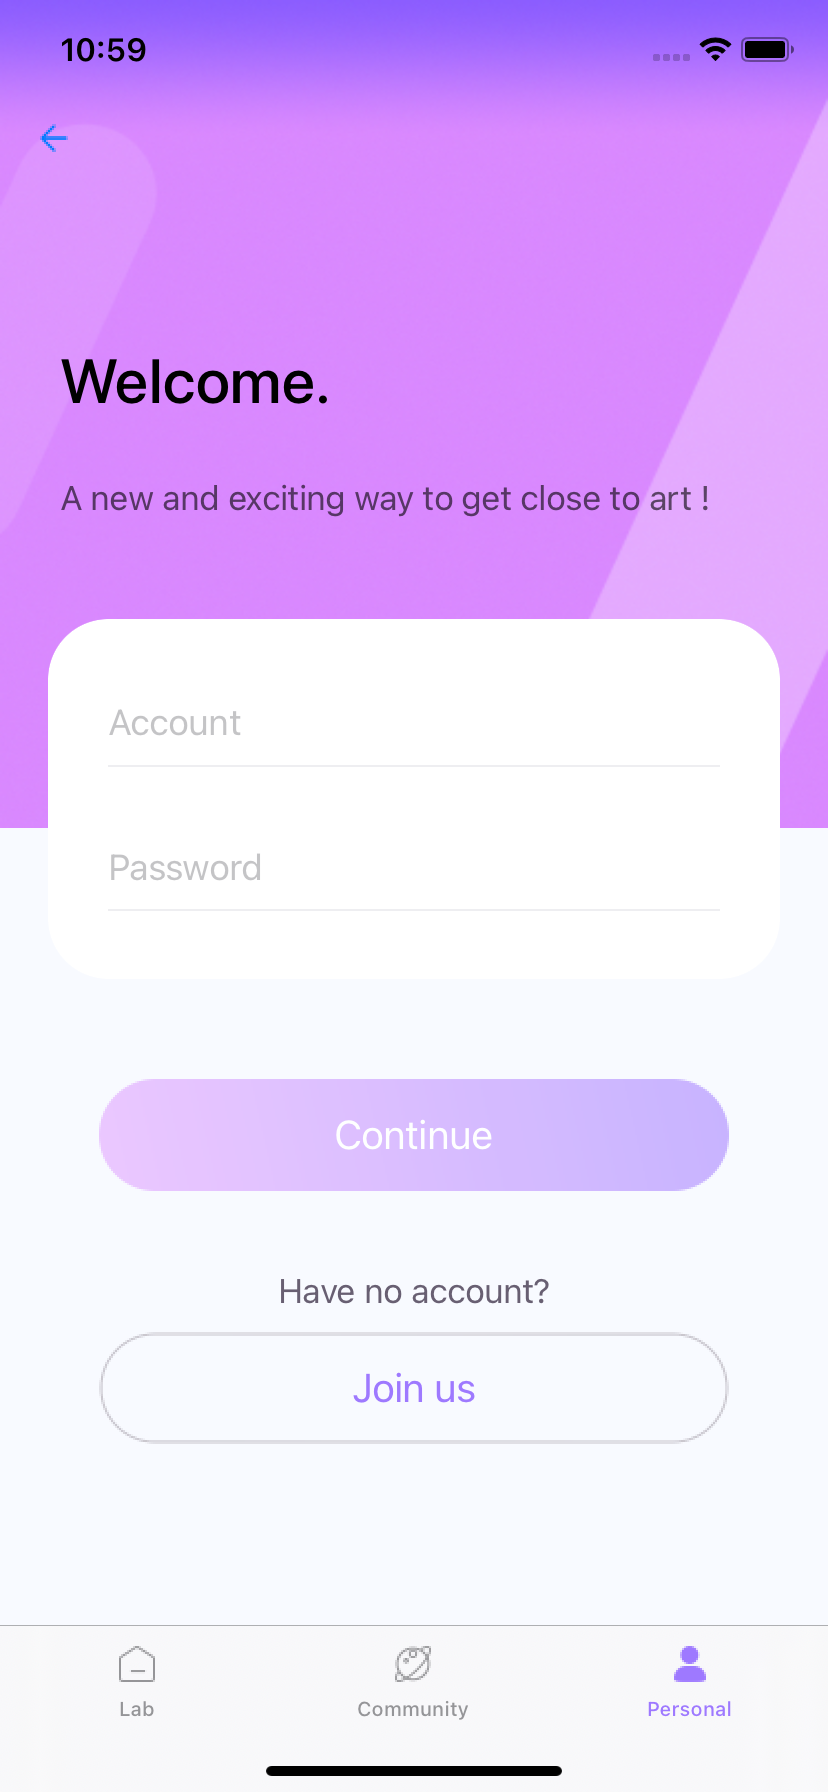
\includegraphics[width=4cm]{figures/登录.png}
\caption{登陆示意图}
\label{fig:my_label}
\end{wrapfigure}

如果用户未登录,点击头像和昵称部分即可进入登录界面。目前已经实现记住账户密码,自动登录功能,并提供了新用户注册入口。用户登录时,App 向服务器发送 POST 请求,将用户名与 HMAC 算法加密后的密码发向服务器,服务器根据登录是否成功,选择返回给 App 用户的唯一标识符,昵称,头像等信息。记住账户密码使用 SAMKeychain 框架,这是对 iOS 原生的安全框架的封装,可以将用户密码加密存储在本地,在便利用户的同时保障了隐私安全。

\subsection{服务器端详细设计}

目前设计的后端主要是和前端相协调,处理事件返回数据。使用 FastAPI 框架基于 Python 语言设计。数据库选择的 MySQL 数据库。首先,利用 FastAPI 框架搭建出最基础的 Web 服务器。采用层次设计的方式进行设计,主要分为 API 层,Service 层,Dao 层以及 NnModel 模块等。

\subsubsection{Dao 层}

Dao 层主要做数据存储层的工作,负责与数据库进行联络的一些类的定义都封装在此,负责业务对象和数据库的关系映射(ORM),Dao 层的设计首先是通过数据库设计好各个数据库,并处理好各个表间的关系,再完成对应关系的转换。

\subsubsection{Service 层}

Service 层主要负责业务模块的应用逻辑应用设计。同样是首先设计接口,再设计其处理对应的函数,接着在配置文件中配置其实现的关联。这样我们就可以在应用中调用函数来进行业务处理。Service 层的业务实际,具体要调用已经定义的 Dao 层所创造好的关系映射,封装 Service 层业务逻辑有利于通用的业务逻辑的独立性和重复利用性。使得程序看上去逻辑清晰。

\subsubsection{API 层}

API 层负责具体的业务模块流程的控制,在此层要调用 Service 层的接口来控制业务流程,控制的配置也同样是在配置文件里进行,针对具体的业务流程,会有不同的控制器。如处理 HTTP 请求和 WebSocket 对应引流到不同的 Service 层中的模块等,这样的设计过程可以将流程进行抽象归纳,设计出可以重复利用的子单元流程模块。使程序结构变得清晰,减少了代码重复使用造成的困扰。

\subsubsection{NnModel 模块}

该模块部署了所需的图像风格迁移模型以及音乐风格迁移模型,前端请求传输到 Service 层时,Service 层根据请求调用NnModel 模块的神经网络模型进行训练,训练完毕后返回风格迁移后的图片或音乐数据。

\subsection{数据库设计}

\subsubsection{需求分析}

App 需要展示个人信息,同时用户需要在社区发帖,收藏别人的帖子以及进行评论等行为,所有本 App 的数据存储工作主要体现在用户的个人信息存储,用户收藏/发布帖子存储和社区帖子评论存储三个方面。

首先是用户的个人信息存储。数据库需要存储每一位用户的用户名和登陆密码以及头像,用户由用户名唯一标识。

其次是用户在社区发布和收藏的帖子信息的存储。App 个人界面需要展示该用户发布的帖子以及收藏的帖子。帖子信息主要包括帖子号,点赞数,音频,图片,文本,日期。帖子由帖子号唯一标识,并以用户名为外键唯一映射到帖子的作者。

最后是用户给帖子的评论信息的存储。评论信息主要包括评论号,文本。评论由评论号唯一标识,通过外键用户名唯一映射到评论者,通过外键帖子号唯一映射到评论对应的帖子。

\subsubsection{概念模型-实体关系图(ER图)设计}

通过需求分析,我们将数据库概念设计的三大实体抽象出来,分别为用户类,评论类和帖子类。三者之间的关系为用户可以发布和收藏帖子,同时可以对帖子进行评论。映射数量上一个用户可以发布或收藏多个帖子,也可以对帖子进行多条评论,因此是 1:N 映射。有了主体,属性和关系,我们设计出如下局部 ER 图和总体 ER 图。

\begin{figure}[H]
    \centering
    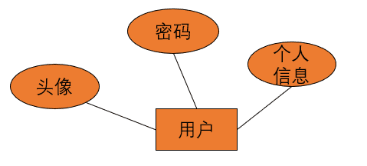
\includegraphics[width=0.6\textwidth]{figures/ER1.png}
    \caption{用户类ER图}
    \label{fig:my_label}
\end{figure}

\begin{figure}[H]
    \centering
    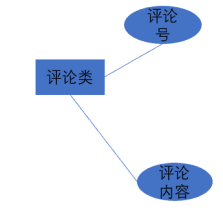
\includegraphics[width=0.6\textwidth]{figures/ER2.png}
    \caption{评论类ER图}
    \label{fig:my_label}
\end{figure}

\begin{figure}[H]
    \centering
    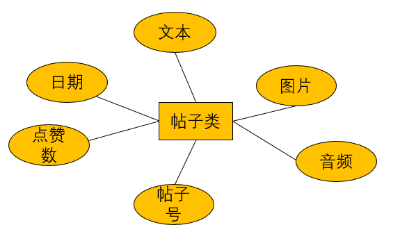
\includegraphics[width=0.6\textwidth]{figures/ER3.png}
    \caption{帖子类ER图}
    \label{fig:my_label}
\end{figure}

\begin{figure}[H]
    \centering
    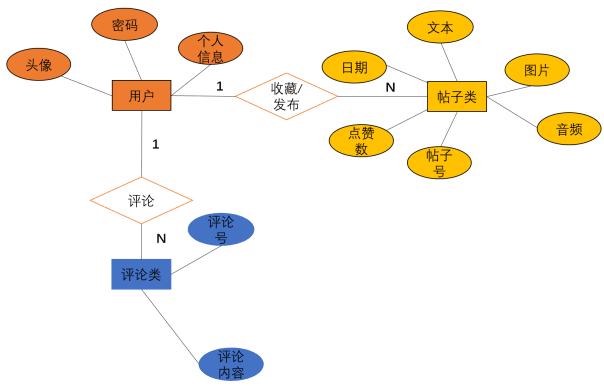
\includegraphics[width=0.8\textwidth]{figures/ER4.png}
    \caption{总体ER图}
    \label{fig:my_label}
\end{figure}